\section{Абстрактная теория меры}
\subsection{Системы множеств}
\begin{definition}
    Пусть $I$~---~индексное множество, $A_\alpha$~---~абстрактное множество $\forall \alpha \in I$. Тогда \textit{системой множеств} назовём совокупность всех $A_\alpha$ и будем обозначать $\{A_\alpha\}_{\alpha \in I}$.
\end{definition}

\begin{lemma}
Пусть $X$~---~абстрактное множество и $\{A_\alpha\}_{\alpha \in I}$~---~система подмножеств $X$, то есть $A_\alpha \subset X$ $\forall \alpha \in I$. Тогда \begin{enumerate}
    \item $X \bs \underset{\alpha \in I}{\bigcup} A_\alpha = \underset{\alpha \in I}{\bigcap} X \bs A_\alpha$
    \item $X \bs \underset{\alpha \in I}{\bigcap} A_\alpha = \underset{\alpha \in I}{\bigcup} X \bs A_\alpha$
    \item $A \cap \underset{\alpha \in I}{\bigcup} A_\alpha = \underset{\alpha \in I}{\bigcup} A \cap A_\alpha$
\end{enumerate}
\end{lemma}

\begin{proof}
    Доказательство состоит в проговаривании смысла равенств.
    
    Лежит в объединении $\Lra$ Лежит хотя бы в одном.
    
    Лежит в пересечении $\Lra$ Лежит в каждом.
\end{proof}

\begin{definition}
    Пусть $A$ и $B$~---~абстрактные множества. Назовём их \textit{симметрической разностью} множество, определяемое равенством $A \vartriangle B := (A \bs B) \cup (B \bs A) = (A \cup B) \bs (A \cap B)$.
\end{definition}

\begin{definition}
    Пусть $\{A_n\}$~---~последовательность множеств. Её \textit{нижним} пределом $\underset{n \ra \infty}{\underline{\lim}} A_n = \underset{n \ra \infty}{\liminf} A_n$ назовём все $x$ такие, что каждый из них принадлежит всем $A_n$, начиная с некоторого номера $N(x)$, то есть 
    \[\forall x \in \underset{n \ra \infty}{\underline{\lim}} A_n \; \exists N(x) \in \N : \forall n \geq N(x) \emb x \in A_n\]
    
    \[\underset{n \ra \infty}{\underline{\lim}} A_n = \overset{\infty}{\underset{N = 1}{\bigcup}} \, \overset{\infty}{\underset{n = N}{\bigcap}}A_n\]
\end{definition}

\begin{definition}
    Пусть $\{A_n\}$~---~последовательность множеств. Её \textit{верхним} пределом $\underset{n \ra \infty}{\overline{\lim}} A_n = \underset{n \ra \infty}{\limsup} A_n$ назовём все $x$ такие, что каждый из них принадлежит бесконечному набору множеств из $\{A_n\}$, то есть 
     \[\forall x \in \underset{n \ra \infty}{\overline{\lim}} A_n \; \forall N \in \N : \exists n(x, N) \geq N \emb x \in A_n\]
    
    \[\underset{n \ra \infty}{\overline{\lim}} A_n = \overset{\infty}{\underset{N = 1}{\bigcap}} \, \overset{\infty}{\underset{n = N}{\bigcup}}A_n\]
\end{definition}

\begin{proposition}
    $\underset{n \ra \infty}{\underline{\lim}} A_n \subset \underset{n \ra \infty}{\overline{\lim}} A_n$\
\end{proposition}

\begin{minipage}{0.5\textwidth}% adapt widths of minipages to your needs
    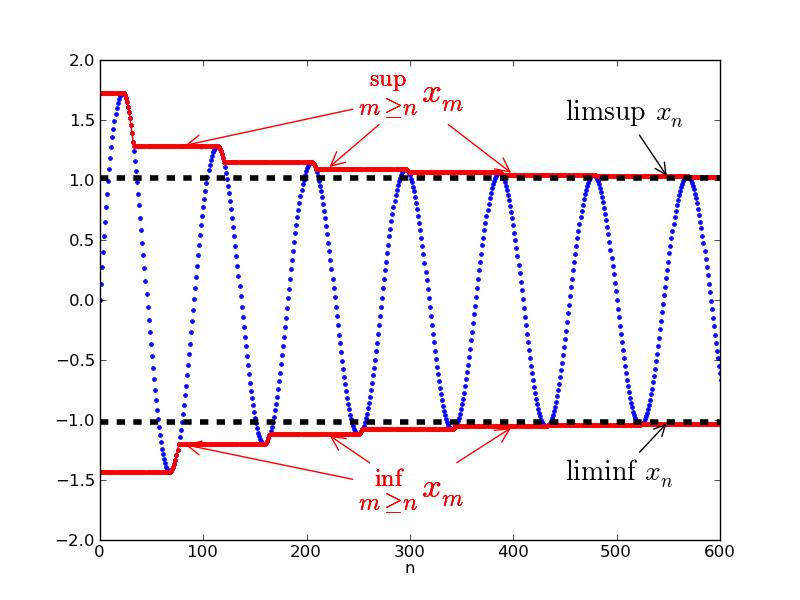
\includegraphics[width=1.0\textwidth]{images/Lim_sup_example_5.png} 
\end{minipage}%
\hfill%
\begin{minipage}{0.5\textwidth}\raggedright
Прим редактора: геометрическая интуиция про эти пределы. Иллюстрация верхнего предела и нижнего предела. Последовательность $\{x_n\}$ показана синим цветом. Две красные кривые приближаются к верхнему пределу и нижнему пределу $\{x_n\}$, показаны пунктирными черными линиями. 
Идея перехода от последовательностей к множествам принадлежит Михаилу Баронову. Представьте теперь что эти числа это размеры шаров(очевидно неотрицательные) с центром в нуле
\end{minipage}
%Зачем эта вставка нужна?

\definition Систему множеств $\Rim$ назовём \textit{кольцом}, если $\forall A, B \in \Rim$ выполнено:
\begin{enumerate}
    \item $A \cup B \in \Rim$;
    \item $A \cap B \in \Rim$;
    \item $A \bs B \in \Rim$.
\end{enumerate}

\definition Будем говорить, что в кольце есть <<единица>>, если $\exists X \in \Rim : A \subset X \; \forall A \in \Rim$

\definition Кольцо с единицей назовём \textit{\textit{алгеброй}}.

\definition Пусть $\A$~---~алгебра с единицей $X$ и $A \in \A$, тогда дополнением $A$ назовём множество $A^c := X \bs A$.

\remark Нетрудно заметить, что для любого кольца $\Rim$ и любой алгебры $\A$ выполняется:
\begin{enumerate}
    \item $\emptyset \in \Rim$;
    \item $A^c \in \A \; \forall A \in \A$;
    \item $\forall A, B \in \Rim \emb A \vartriangle B \in \Rim$.
\end{enumerate}

На самом деле, для определения кольца достаточно было использовать только пересечение и симметрическую разность, потому что объединение и вычитание выражаются через них:

\begin{enumerate}
    \item[$\bullet$] $A \bs B = A \cap B^c$;
    \item[$\bullet$] $A \cup B = (A \Delta B) \ \Delta \ (A \cap B) $.
\end{enumerate}

\definition Алгебра $\A$ называется {\textit{$\sigma$-алгеброй}}, если $\forall \text{ последовательности } \{A_n\} \subset \A \emb \underset{n = 1}{\overset{\infty}{\bigcup}} A_n \in \A$.

\remark Для $\sigma$-алгебры также верно, что любое счётное пересечение в ней лежит (это верно в силу закона двойственности).
\hypertarget{TrivialSigma}{}
\example Тривиальные $\sigma$-алгебры: $\{\emptyset, X\}$, $2^X$.

\hypertarget{minimalSigmaAlgebra}{}
\lemma Пусть $\{\A_\alpha\}_{\alpha \in I}$ - семейство алгебр, с <<единицей>> $X$. Тогда $\underset{\alpha \in I}{\bigcap} \A_\alpha = \A$ - алгебра с единицей $X$.

\begin{proof}
    $X$~---~<<единица>>, для всех алгебр из семейства $\Ra X \in \underset{\alpha \in I}{\bigcap} \A_\alpha$. 
    
    Покажем, что $\forall A, B \in \underset{\alpha \in I}{\bigcap} \A_\alpha \emb A \bs B, A \cap B, A \cup B \in \underset{\alpha \in I}{\bigcap} \A_\alpha$
    $$A, B \in \underset{\alpha \in I}{\bigcap} \A_\alpha \Ra \forall \alpha \in I \emb A, B \in \A_\alpha \Ra A \bs B, A \cap B, A \cup B \in \A_\alpha \; \forall \alpha \in I \Ra A \bs B, A \cap B, A \cup B \in \underset{\alpha \in I}{\bigcap} \A_\alpha.$$
\end{proof}

\remark Аналогично доказывается то же утверждение, но для семейства $\sigma$-алгебр, с общей <<единицей>> $X$.

% Тож поправить
\theorem $\forall$ системы $\E$ подмножеств множества $X$ существует и единственна наименьшая по включению $\sigma$-алгебра, содержащая $\E$. То есть, \textit{$\sigma$-алгебра, порождённая $\E$}, и обозначается $\M(\E)$.

\begin{proof}
Разобьём доказательство на шаги.
\begin{itemize}
    \item \textbf{Существование}.

    Рассмотрим семейство всех $\sigma$-алгебр, содержащих $\E$, обозначим его $\{\M_\alpha\}_{\alpha \in I}$. Это семейство не пусто, потому что в нём есть хотя бы \hyperlink{TrivialSigma}{один тривиальный пример}.
    
    Положим $\M(\E) = \underset{\alpha \in I}{\bigcap} \M_\alpha$. Оно является $\sigma$-алгеброй по \hyperlink{minimalSigmaAlgebra}{лемме}. Также оно содержит $\E$, поскольку $\E \subset \M_\alpha \; \forall \alpha \in I$. 
    
    \item \textbf{Минимальность}.

    Пусть есть $\M'$~---~$\sigma$-алгебра, содержащая $\E$. Но так как она содержит $\E$, то $\exists \alpha' \in I$: $\M' = \M_{\alpha'}$. Но $\underset{\alpha \in I}{\bigcap} \M_\alpha \subset \M_{\alpha'}$. Значит она минимальна.

    \item \textbf{Единственность}.

    Если бы их было две, то первая должна содержать вторую и вторая первую, значит они равны.
\end{itemize}
\end{proof}
\begin{note}
    Данная процедура пополнения неконструктивная для бесконечных множеств. Мы не предъявили алгоритм построения, а лишь доказали существование.
\end{note}

\begin{example}
Рассмотрим абстрактное множество $X$. Пусть $A_0, A_1, \dots, A_{n-1}, n \in \N$~---~набор подмножеств $X$, где $A_0 := X$.
% Это обозначение я тоже не понимаю
Рассмотрим всевозможные наборы $\epsilon = (0, 1, 1, 0, \dots, 0)$ из $0$ и $1$. $A_\epsilon = \underset{k = 0}{\overset{n - 1}{\bigcap}} A_k^{\epsilon_k}$. Теперь составим нашу систему $\M$ из $A_\epsilon$ и их всевозможных объединений. Это и будет $\sigma$-алгеброй. В ней $\leq 2^{2^n}$ элементов.
\end{example}

\definition Если $(X, \rho)$~---~метрическое пространство, то $\B(X)$~---~\textit{борелевская $\sigma$-алгебра}, то есть наименьшая $\sigma$-алгебра, содержащая все открытые множества в $X$.

\remark Сам по себе набор открытых множеств не образует алгебру. Если мы возьмём в качестве метрического пространства $(\R, \|\cdot\|)$ и рассмотрим интервал $A = (0, 1)$, то $A^c = \R \bs A$ - не открыто.
%Пу-пу-пу...
\remark Борелевские подмножества~---~это не все подмножества. Мощность борелевской системы в $\R^n$ континуальна, а множество всех подмножеств гиперконтинуально
\remark Непрерывное отображение борелевского не всегда борелевское. Но это за пределами программы. Кому интересно см. Суслинские множества

\examples Пусть $X$~---~абстрактное множество.
\begin{enumerate}
    \item $\{\emptyset, X\}$ - $\sigma$-алгебра;
    \item $2^X$ - семейство подмножеств $X$ является $\sigma$-алгеброй;
    \item $\M$ - все такие подмножества числовой прямой, что-либо оно счётно, либо его дополнение не более чем счётно. Это также является $\sigma$-алгеброй;
    \item $\M$ - все такие подмножества числовой прямой, что-либо оно, либо его дополнение не более чем конечно. Это является алгеброй, но не $\sigma$-алгеброй.
\end{enumerate}

\definition Система множеств $\PP$ называется \textit{полукольцом}, если:

\begin{enumerate}
    \item $\emptyset \in \PP$;
    \item $\forall A, B \in \PP \hookrightarrow A \cap B \in \PP$;
    \item $\forall A, B \in \PP$ $A \bs B = \overset{N}{\underset{n = 1}{\bigsqcup}} A_n$, где $A_n \in \PP$.
\end{enumerate}

\remark В определении полукольца мы не требуем что работаем с подмножествами какого-то большого множества, это просто система множеств
\example Приведём пример полукольца (даже с единицей), но не кольца: $$X = [a, b), \quad \PP = \{[\alpha, \beta) : a \leq \alpha \leq \beta \leq b\}.$$ 

(Доказательство оставлено читателю в качестве упражнения)

\lemma Если $\{A_n\}_{n = 1}^{\infty}$~---~произвольная последовательность множеств, тогда их объединение можно представить в виде дизъюнктного, то есть $\overset{\infty}{\underset{n = 1}{\bigcup}} A_n = \overset{\infty}{\underset{n = 1}{\bigsqcup}} C_n$, где $C_n := A_n \bs \overset{n-1}{\underset{k = 1}{\bigcup}} A_k$, $C_1 = A_1$

\begin{proof} Покажем включение в обе стороны:

\begin{itemize}
    \item $\overset{\infty}{\underset{n = 1}{\bigsqcup}} C_n \subset \overset{\infty}{\underset{n = 1}{\bigcup}} A_n$, поскольку $\forall n \in \N \; C_n \subset A_n$
    
    \item $\overset{\infty}{\underset{n = 1}{\bigcup}} A_n \subset \overset{\infty}{\underset{n = 1}{\bigsqcup}} C_n$

    $\forall x \in \overset{\infty}{\underset{n = 1}{\bigcup}} A_n\;$ $\;m_x := \min\{n \in N\text{: } x \in A_n\}, m_0 := \emptyset$

    Из определения $m_x$, следует: $x \notin A_m \; \forall m < m_x \Ra x \in A_{m_x} \bs \bigcup\limits_{k = 1}^{m_x - 1} A_k \Ra x \in C_{m_x} \Ra \overset{\infty}{\underset{n = 1}{\bigcup}} A_n \subset \overset{\infty}{\underset{n = 1}{\bigsqcup}} C_n$
\end{itemize}
\end{proof}
\hypertarget{disjoint_union}{}
\theorem (Теорема о дизъюнктном разбиении) Пусть $\PP$ - полукольцо, а $P, P_1, \dots, P_n \in \PP, n \in \N$. Тогда

\begin{enumerate}
    \item $\forall n \in \N \ \exists$ конечное семейство попарно непересекающихся множеств $Q_1, \dots, Q_m \in \PP$, т.ч. $P \bs \overset{n}{\underset{k = 1}{\bigcup}} P_k = \overset{m}{\underset{i = 1}{\bigsqcup}} Q_i$
    \item $\forall n \in \N, n \geq 2 \ \exists R_k \in \PP \; (k = 1, \dots, N)$, т.ч. $\overset{n}{\underset{i = 1}{\bigcup}} P_i = \overset{N}{\underset{k = 1}{\bigsqcup}} R_k$. При этом $\forall k \in \{1, \dots, N\}$ и $\forall i \in \{1, \dots, n\}$, либо $R_k \subset P_i$, либо $R_k \cap P_i = \emptyset$ (*)
\end{enumerate}
\remark Первый пункт теоремы нетривиален, как могло показаться, ведь по определению 
то выполнено, для $n=1$, но вот $\overset{n}{\underset{k = 1}{\bigcup}} P_k$ не обязательно лежит в полукольце. Тем не менее мы можем дополнить элементами полукольца

\begin{proof} Рассмотрим доказательство каждого пункта по отдельности
\begin{enumerate}
    \item Докажем по индукции.
    
    \begin{itemize}
        \item \textbf{База:} Для $n = 1$ утверждение следует из определения полукольца.
        \item \textbf{Предположение:} Пусть утверждение доказано при $n = l$.
        \item \textbf{Шаг:} Докажем для $n = l + 1$.

        $P \bs (P_1 \cup \dots \cup P_l) = \overset{m}{\underset{i = 1}{\bigsqcup}}Q_i$, где $Q_i \in \PP$

        В силу закона двойственности: 

        $P \bs (P_1 \cup \dots \cup P_l \cup P_{l+1}) = (P \bs P_{l + 1}) \cap (P \bs (P_1 \cup \dots \cup P_l))$

        $P \bs P_{l + 1} = \overset{k}{\underset{j = 1}{\bigsqcup}} S_j$, где $S_j \in \PP$

        Рассмотрим, всевозможные пересечения $Q_i \cap S_j$.
        
        Тогда $(P \bs P_{l + 1}) \cap (P \bs (P_1 \cup \dots \cup P_l)) = (\overset{k}{\underset{j = 1}{\bigsqcup}} S_j) \cap (\overset{m}{\underset{i = 1}{\bigsqcup}} Q_i) = \overset{k}{\underset{j = 1}{\bigsqcup}}\overset{m}{\underset{i = 1}{\bigsqcup}} S_j \cap Q_i$

        Так как $S_j, Q_i \in \PP \Ra S_j \cap Q_i \in \PP$. Следовательно, сделав шаг индукции, мы получили конечное дизъюнктное разбиение для $n = l + 1$. Значит доказательство по индукции выполнено.
    \end{itemize}

    \item Докажем по индукции.
    
    \begin{itemize}
        \item \textbf{База:} Для $n = 2$: $P_1 \cup P_2 = (P_1 \bs P_2) \sqcup (P_1 \cap P_2) \sqcup (P_2 \bs P_1) = \overset{m}{\underset{i = 1}{\bigsqcup}}Q_i \sqcup (P_1 \cap P_2) \sqcup \overset{l}{\underset{j = 1}{\bigsqcup}}S_j$
        \item \textbf{Предположение:} Пусть доказали при $n \leq n'$.
        \item \textbf{Шаг:} Докажем для $n' + 1$. Очевидно, что $\overset{n' + 1}{\underset{i = 1}{\bigcup}}P_i = P_{n' + 1} \cup \overset{n'}{\underset{i = 1}{\bigcup}}P_i$

        Рассмотрим множества $I_1 = P_{n' + 1} \bs \overset{n'}{\underset{i = 1}{\bigcup}}P_i$, $I_2 = P_{n' + 1} \cap \overset{n'}{\underset{i = 1}{\bigcup}}P_i$, $I_3 = \overset{n'}{\underset{i = 1}{\bigcup}}P_i \bs P_{n' + 1}$. Тогда $I_1 \cup I_2 \cup I_3 = P_{n' + 1} \cup \overset{n'}{\underset{i = 1}{\bigcup}}P_i$

        Из первого пункта теоремы следует, что $I_1 = \overset{l}{\underset{j = 1}{\bigsqcup}}S_j$, где $S_j \in \PP$ при каждом $j$.

        По предположению индукции: $I_2 = P_{n' + 1} \cap \overset{n'}{\underset{i = 1}{\bigcup}}P_i = P_{n' + 1} \cap \overset{N}{\underset{k = 1}{\bigsqcup}} R_k = \overset{N}{\underset{k = 1}{\bigsqcup}} (R_k \cap P_{n' + 1})$, из определения полукольца $R_k \cap P_{n' + 1} \in \PP$.

        По предположению индукции: $I_3 = \overset{n'}{\underset{i = 1}{\bigcup}}P_i \bs P_{n' + 1} = \overset{N}{\underset{k = 1}{\bigsqcup}} R_k \bs P_{n' + 1} = \overset{N}{\underset{k = 1}{\bigsqcup}} (R_k \bs P_{n' + 1})$, из определения полукольца $R_k \bs P_{n' + 1} = \overset{m}{\underset{t = 1}{\bigsqcup}} M_t$ $\forall k \in \{1, \dots, N\}$, где $M_t \in \PP$.

        Заметим, что $I_1 \cap I_2 = I_2 \cap I_3 = I_3 \cap I_1 = \emptyset$. Таким образом мы разложили три не пересекающихся множества в дизъюнктные объединения, значит мы всё это собираем вместе, нумеруем единым индексом и получаем то, что хотели.
    \end{itemize}
    Свойство (*) видно из построения. Очевидно, что $R_k \bs P_{n' + 1} \nsubseteq P_{n' + 1}, \; R_k \bs P_{n' + 1} \subset R_k \Ra R_k \bs P_{n' + 1} \subset P_q$, для какого-то $q < n$. А для $n$ уже доказано (предположение индукции).
\end{enumerate}
\end{proof}

\definition Пусть $\PP_1, \PP_2$ - полукольца. Определим их \textit{тензорное произведение} $\PP_1 \otimes \PP_2 := \{P \times Q : P \in \PP_1, Q \in \PP_2\}$. Произведение пустых по определению положим пустым.

\theorem Пусть $\PP_1, \PP_2$ - полукольца, тогда $\PP_1 \otimes \PP_2$ - тоже полукольцо.

\begin{proof} Докажем все свойства из определения полукольца по порядку.

\begin{enumerate}
\item \textit{Свойство 1.} $\emptyset \times \emptyset = \emptyset$

\item \textit{Свойство 2.} Теперь докажем, что пересечение тоже лежит в произведении

$(C_1 \times D_1) \cap (C_2 \times D_2) = (C_1 \cap C_2) \times (D_1 \cap D_2)$.

\item \textit{Свойство 3.}

Рассмотрим $A \in \PP_1$ и $B \in \PP_2$ и $E \subset A \times B$ при $E \in \PP_1 \otimes \PP_2$.

Т.к. $E \in \PP_1 \otimes \PP_2$, то $\exists C \in \PP_1$ и $\exists D \in \PP_2$, т.ч. $C \times D = E$.

Из определения полукольца следует, что $A \bs C = \bigsqcup\limits_{i = 1}^{N} A_i, \;\; A_i \in \PP_1$.

Также, из определения полукольца следует, что $B \bs D = \bigsqcup\limits_{j = 1}^{L} B_j, \;\; B_j \in \PP_2$.

Дополнительно определим $A_0 := C$ и $B_0 := D$

Определим $F_{ij} := A_i \times B_j$. Из определения тензорного произведения $F_{ij} \in \PP_1 \otimes \PP_2$

Заметим, что $F_{ij} \cap F_{i^*j^*} = \emptyset$, при $(i, j) \neq (i^*, j^*)$ 

Значит $A \times B = \bigsqcup\limits_{i, j = 0}^{N, L} F_{ij} \Ra (A \times B) \bs (C \times D) = \bigsqcup\limits_{i, j = 0, \ (i, j) \neq (0, 0)}^{N, L} F_{ij}$ 
\end{enumerate}
\end{proof}

\corollary Эта конструкция будет часто использоваться. Пусть

$a = (a_1, \dots, a_n) \in \R^n$

$b = (b_1, \dots, b_n) \in \R^n$

и $[a, b) := \prod\limits_{i= 1}^{n}[a_i, b_i)$ $b_i \geq a_i \; \forall i$

Тогда система всех $[\alpha, \beta)$ содержащихся в $[a, b)$ (где $\alpha = (\alpha_1, \dots, \alpha_n)$, и $\beta = (\beta_1, \dots, \beta_n)$ $\beta_i \geq \alpha_i \; \forall i$) образует полукольцо с единицей $[a, b)$

\proposition Любое открытое множество в $\R^n$ можно представить, как не более чем счётное объединение полуоткрытых параллелепипедов с рациональными вершинами.

% Ну дополним.
\begin{proof}
Оставляется в качестве упражнения читателю (есть в Макарове-Подкорытове)
\end{proof}

\subsection{Свойства полуколец}

\definition Пусть $\PP$~---~полукольцо. Тогда отображение $\mu$: $\PP \ra [0, +\infty]$ называется конечно-аддитивной мерой, если:

\begin{enumerate}
    \item $\mu (\emptyset) := 0$;
    \item Если $C \in \PP$ и $C = \overset{n}{\underset{k = 1}{\bigsqcup}} Q_k, \; Q_k \in \PP$, тогда $\mu(C) = \overset{n}{\underset{k = 1}{\sum}} \mu(Q_k)$.
\end{enumerate}
% Это вообще какая-то хуйня...
%\begin{note}
%    Если $\mu: \PP \rightarrow [0, +\infty)$~---~мера, то %она называется конечной мерой.
%\end{note}
\lemma Пусть $\PP$~---~полукольцо, $\mu$~---~мера на $\PP$, тогда верны следующие свойства:

\begin{enumerate}
    \item \textit{Монотонность:} $\forall A, B \in \PP, \; A \subset B \Ra \mu(A) \leq \mu(B)$;
    \item \textit{Продвинутая монотонность:} Если $A \in \PP$ и $A_1, \dots, A_n \in \PP$ - попарно не пересекаются и $A_i \subset A \; \forall i$, то $\sum\limits_{i = 1}^{n}\mu(A_i) \leq \mu(A)$;
    \item \textit{Полуаддитивность:} Если $B \in \PP, B \subset \bigcup\limits_{i = 1}^{n} A_i$ и $\ A_i \in \PP$ при всех $i \in \{1, \ldots, n\}$, то $\mu(B) \leq \sum\limits_{i = 1}^{n} \mu(A_i)$.
\end{enumerate}

\begin{proof} Докажем пункты по порядку.
%Поправить.
\begin{enumerate}
    \item Следует из 2).
    \item \hyperlink{disjoint_union}{Из теоремы о дизъюнктом разбиении} $A \bs \bigsqcup\limits_{i = 1}^{n} A_i = \bigsqcup\limits_{k = 1}^{N} Q_k \Ra A = (\bigsqcup\limits_{i = 1}^{n} A_i) \sqcup (\bigsqcup\limits_{k = 1}^{N} Q_k)$. Значит, из свойств меры получим $\mu(A) = \sum\limits_{i = 1}^{n}\mu(A_i) + \sum\limits_{k = 1}^{N}\mu(Q_k)$, но так как $\mu(Q_k) \geq 0$, то $\sum\limits_{k = 1}^{N}\mu(Q_k) \geq 0 \Ra \sum\limits_{i = 1}^{n}\mu(A_i) \leq \mu(A)$
    \item Заметим, что $B \cap A_i \in \PP$, и при этом, так как $\PP$ - полукольцо, $B \bs A_i = \bigsqcup\limits_{j = 1}^{m_i} Q_{i,j}$, где $Q_{i, j} \in \PP \; \forall i, j$

    Тогда по определению меры $\mu(A_i) = \mu(B \cap A_i) + \sum\limits_{j = 1}^{m_i}\mu(Q_{i, j}) \; \forall i$

    %TODO

    %ЭТО НЕ ПРАВДА $\mu(B) = \mu(B \cap A_i) + \sum\limits_{j = 1}^{m_i}\mu(Q_{i, j}) = \mu(B \cap A_i) + \mu(B \bs A_i)$

    
    
\end{enumerate}
\end{proof}